%%
%% Automatically generated file from DocOnce source
%% (https://github.com/doconce/doconce/)
%% doconce format latex UiOdiscussionsMarch4.do.txt --latex_title_layout=beamer --latex_table_format=footnotesize --no_mako
%%
% #ifdef PTEX2TEX_EXPLANATION
%%
%% The file follows the ptex2tex extended LaTeX format, see
%% ptex2tex: https://code.google.com/p/ptex2tex/
%%
%% Run
%%      ptex2tex myfile
%% or
%%      doconce ptex2tex myfile
%%
%% to turn myfile.p.tex into an ordinary LaTeX file myfile.tex.
%% (The ptex2tex program: https://code.google.com/p/ptex2tex)
%% Many preprocess options can be added to ptex2tex or doconce ptex2tex
%%
%%      ptex2tex -DMINTED myfile
%%      doconce ptex2tex myfile envir=minted
%%
%% ptex2tex will typeset code environments according to a global or local
%% .ptex2tex.cfg configure file. doconce ptex2tex will typeset code
%% according to options on the command line (just type doconce ptex2tex to
%% see examples). If doconce ptex2tex has envir=minted, it enables the
%% minted style without needing -DMINTED.
% #endif

% #define PREAMBLE

% #ifdef PREAMBLE
%-------------------- begin preamble ----------------------

\documentclass[%
oneside,                 % oneside: electronic viewing, twoside: printing
final,                   % draft: marks overfull hboxes, figures with paths
10pt]{article}

\listfiles               %  print all files needed to compile this document

\usepackage{relsize,makeidx,color,setspace,amsmath,amsfonts,amssymb}
\usepackage[table]{xcolor}
\usepackage{bm,ltablex,microtype}

\usepackage[pdftex]{graphicx}

\usepackage[T1]{fontenc}
%\usepackage[latin1]{inputenc}
\usepackage{ucs}
\usepackage[utf8x]{inputenc}

\usepackage{lmodern}         % Latin Modern fonts derived from Computer Modern

% Hyperlinks in PDF:
\definecolor{linkcolor}{rgb}{0,0,0.4}
\usepackage{hyperref}
\hypersetup{
    breaklinks=true,
    colorlinks=true,
    linkcolor=linkcolor,
    urlcolor=linkcolor,
    citecolor=black,
    filecolor=black,
    %filecolor=blue,
    pdfmenubar=true,
    pdftoolbar=true,
    bookmarksdepth=3   % Uncomment (and tweak) for PDF bookmarks with more levels than the TOC
    }
%\hyperbaseurl{}   % hyperlinks are relative to this root

\setcounter{tocdepth}{2}  % levels in table of contents

% Tricks for having figures close to where they are defined:
% 1. define less restrictive rules for where to put figures
\setcounter{topnumber}{2}
\setcounter{bottomnumber}{2}
\setcounter{totalnumber}{4}
\renewcommand{\topfraction}{0.95}
\renewcommand{\bottomfraction}{0.95}
\renewcommand{\textfraction}{0}
\renewcommand{\floatpagefraction}{0.75}
% floatpagefraction must always be less than topfraction!
% 2. ensure all figures are flushed before next section
\usepackage[section]{placeins}
% 3. enable begin{figure}[H] (often leads to ugly pagebreaks)
%\usepackage{float}\restylefloat{figure}

\usepackage[framemethod=TikZ]{mdframed}

% --- begin definitions of admonition environments ---

% Admonition style "mdfbox" is an oval colored box based on mdframed
% "notice" admon
\colorlet{mdfbox_notice_background}{gray!5}
\newmdenv[
  skipabove=15pt,
  skipbelow=15pt,
  outerlinewidth=0,
  backgroundcolor=mdfbox_notice_background,
  linecolor=black,
  linewidth=2pt,       % frame thickness
  frametitlebackgroundcolor=mdfbox_notice_background,
  frametitlerule=true,
  frametitlefont=\normalfont\bfseries,
  shadow=false,        % frame shadow?
  shadowsize=11pt,
  leftmargin=0,
  rightmargin=0,
  roundcorner=5,
  needspace=0pt,
]{notice_mdfboxmdframed}

\newenvironment{notice_mdfboxadmon}[1][]{
\begin{notice_mdfboxmdframed}[frametitle=#1]
}
{
\end{notice_mdfboxmdframed}
}

% Admonition style "mdfbox" is an oval colored box based on mdframed
% "summary" admon
\colorlet{mdfbox_summary_background}{gray!5}
\newmdenv[
  skipabove=15pt,
  skipbelow=15pt,
  outerlinewidth=0,
  backgroundcolor=mdfbox_summary_background,
  linecolor=black,
  linewidth=2pt,       % frame thickness
  frametitlebackgroundcolor=mdfbox_summary_background,
  frametitlerule=true,
  frametitlefont=\normalfont\bfseries,
  shadow=false,        % frame shadow?
  shadowsize=11pt,
  leftmargin=0,
  rightmargin=0,
  roundcorner=5,
  needspace=0pt,
]{summary_mdfboxmdframed}

\newenvironment{summary_mdfboxadmon}[1][]{
\begin{summary_mdfboxmdframed}[frametitle=#1]
}
{
\end{summary_mdfboxmdframed}
}

% Admonition style "mdfbox" is an oval colored box based on mdframed
% "warning" admon
\colorlet{mdfbox_warning_background}{gray!5}
\newmdenv[
  skipabove=15pt,
  skipbelow=15pt,
  outerlinewidth=0,
  backgroundcolor=mdfbox_warning_background,
  linecolor=black,
  linewidth=2pt,       % frame thickness
  frametitlebackgroundcolor=mdfbox_warning_background,
  frametitlerule=true,
  frametitlefont=\normalfont\bfseries,
  shadow=false,        % frame shadow?
  shadowsize=11pt,
  leftmargin=0,
  rightmargin=0,
  roundcorner=5,
  needspace=0pt,
]{warning_mdfboxmdframed}

\newenvironment{warning_mdfboxadmon}[1][]{
\begin{warning_mdfboxmdframed}[frametitle=#1]
}
{
\end{warning_mdfboxmdframed}
}

% Admonition style "mdfbox" is an oval colored box based on mdframed
% "question" admon
\colorlet{mdfbox_question_background}{gray!5}
\newmdenv[
  skipabove=15pt,
  skipbelow=15pt,
  outerlinewidth=0,
  backgroundcolor=mdfbox_question_background,
  linecolor=black,
  linewidth=2pt,       % frame thickness
  frametitlebackgroundcolor=mdfbox_question_background,
  frametitlerule=true,
  frametitlefont=\normalfont\bfseries,
  shadow=false,        % frame shadow?
  shadowsize=11pt,
  leftmargin=0,
  rightmargin=0,
  roundcorner=5,
  needspace=0pt,
]{question_mdfboxmdframed}

\newenvironment{question_mdfboxadmon}[1][]{
\begin{question_mdfboxmdframed}[frametitle=#1]
}
{
\end{question_mdfboxmdframed}
}

% Admonition style "mdfbox" is an oval colored box based on mdframed
% "block" admon
\colorlet{mdfbox_block_background}{gray!5}
\newmdenv[
  skipabove=15pt,
  skipbelow=15pt,
  outerlinewidth=0,
  backgroundcolor=mdfbox_block_background,
  linecolor=black,
  linewidth=2pt,       % frame thickness
  frametitlebackgroundcolor=mdfbox_block_background,
  frametitlerule=true,
  frametitlefont=\normalfont\bfseries,
  shadow=false,        % frame shadow?
  shadowsize=11pt,
  leftmargin=0,
  rightmargin=0,
  roundcorner=5,
  needspace=0pt,
]{block_mdfboxmdframed}

\newenvironment{block_mdfboxadmon}[1][]{
\begin{block_mdfboxmdframed}[frametitle=#1]
}
{
\end{block_mdfboxmdframed}
}

% --- end of definitions of admonition environments ---

% prevent orhpans and widows
\clubpenalty = 10000
\widowpenalty = 10000

% --- end of standard preamble for documents ---


% insert custom LaTeX commands...

\raggedbottom
\makeindex

%-------------------- end preamble ----------------------

\begin{document}

% matching end for #ifdef PREAMBLE
% #endif

\newcommand{\exercisesection}[1]{\subsection*{#1}}


% ------------------- main content ----------------------



% ----------------- title -------------------------

\title{Discussions on SFIs, Machine Learning and Artificial Intelligence, Quantum Technologies and more}

% ----------------- author(s) -------------------------

\author{Department of Physics, UiO\inst{}}
\institute{}
% ----------------- end author(s) -------------------------
% at Department of Physics and Astronomy and FRIB, Michigan State University, USA, and Department of Physics and Center for Computing in Science Education,
% University of Oslo, Norway

\date{Mar 4, 2024
% <optional titlepage figure>
% <optional copyright>
}

% !split
\subsection{Background}

The Research Council of Norway released on February 8, 2024, a notice about new centers for innovation.
In the \href{{https://www.forskningsradet.no/forskningspolitikk-strategi/ltp/kunstig-intelligens/}}{original timeline}, a tentative deadline for calls was end of February 2024.

% !split
\subsection{Summary from press release Feb 8 (in Norwegian)}

\begin{enumerate}
\item AI-milliarden skal i hovedsak innrettes som utfordringsrettede sentra for kunstig intelligens.

\item Det skal utlyses 4-6 femårige, tverrfaglige og tverrsektorielle KI-sentre innenfor en ramme på 850 MNOK. Sentra kan ha ulik størrelse.

\item Disponering av resterende midler kan for eksempel omfatte forskerskoler, internasjonalt samarbeid og koordinering.
\end{enumerate}

\noindent
Styret ber administrasjonen og porteføljestyret identifisere muligheter for supplerende finansiering av sentrene og av satsingen.
Styret ber administrasjonen foreslå mekanismer for koordinering, dialog, nasjonal og internasjonal synlighet av norsk KI-forskning og KI-innovasjon, og legge dette frem for Styret medio 2024.

% !split
\subsection{Three main paths}

\begin{enumerate}
\item Research into the consequences of artificial intelligence and other digital technologies for society. Central themes will be democracy, trust, ethics, economy, legal certainty, legal regulations, privacy, \textbf{teaching and learning}, arts and culture.

\item Digital technologies as a research area in itself, i.e. \textbf{research into artificial intelligence}, \textbf{digital security}, \textbf{next generation information technologies}, \textbf{new sensors and quantum technologies}.

\item Research on how digital technologies can be used for \textbf{innovation} in business and the public sector and how \textbf{artificial intelligence can be used in research in different disciplines}
\end{enumerate}

\noindent
% !split
\subsection{Educational initiatives and international cooperation}

In addition to the AI centers, 150 MNOK will go to other things. This
can for example include research schools, international cooperations
and coordinations.

% !split
\subsection{What can it be?}

\textbf{Center for Artificial Intelligence and Quantum Technology (CAIQT)}

Artificial intelligence and quantum technology are revolutionizing our
life and work. They offer enormous advantages for science, economy,
politics and civil society.
The challenges and opportunities in the field of artificial
intelligence and quantum technology call for new kinds of cooperation and new research directions.

% !split
\subsection{Our strengths}

\begin{block}{Several research activities on AI/ML for the physical sciences }
\begin{enumerate}
\item Research, applications and development of new methods in AI/ML

\item Research and development of quantum information science/technologies

\item Strong educational and training activities across disciplines

\item Many national and international collaborations across disciplines
\end{enumerate}

\noindent
\end{block}

\begin{itemize}
\item Partners at UiO: Math, Informatics, Chemistry, Bioscience, Geoscience, ITA, DScience

\item Partners and collaborators outside UiO: CERN, SINTEF, OsloMet, SIMULA, Bank of Norway, DNB,  Norwegian Meteorological Institute and more
\end{itemize}

\noindent
% !split
\subsection{AI/Machine learning. A simple perspective on the interface between ML and Physics}

\vspace{6mm}

% inline figure
\centerline{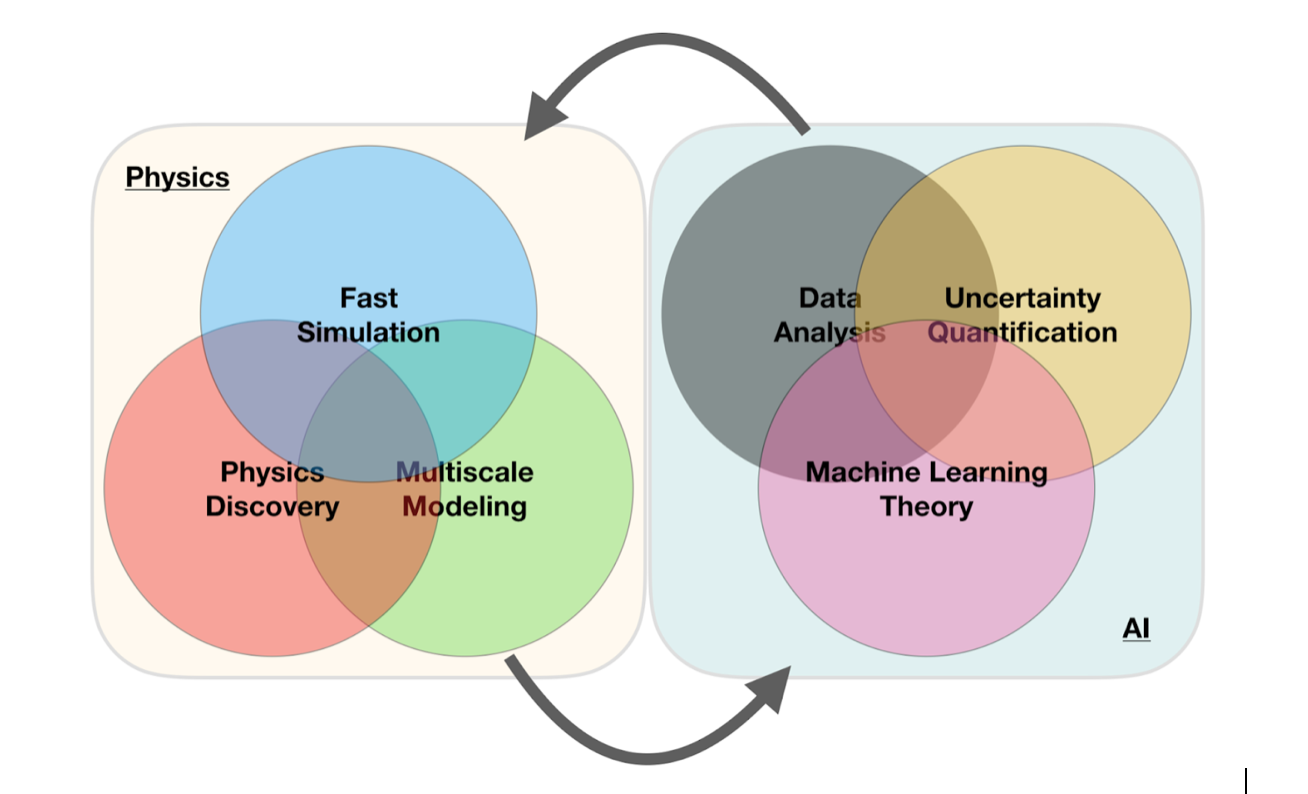
\includegraphics[width=1.0\linewidth]{figures/mlimage.png}}

\vspace{6mm}

% !split
\subsection{AI/ML in Nuclear  Physics (or any field in physics)}

\vspace{6mm}

% inline figure
\centerline{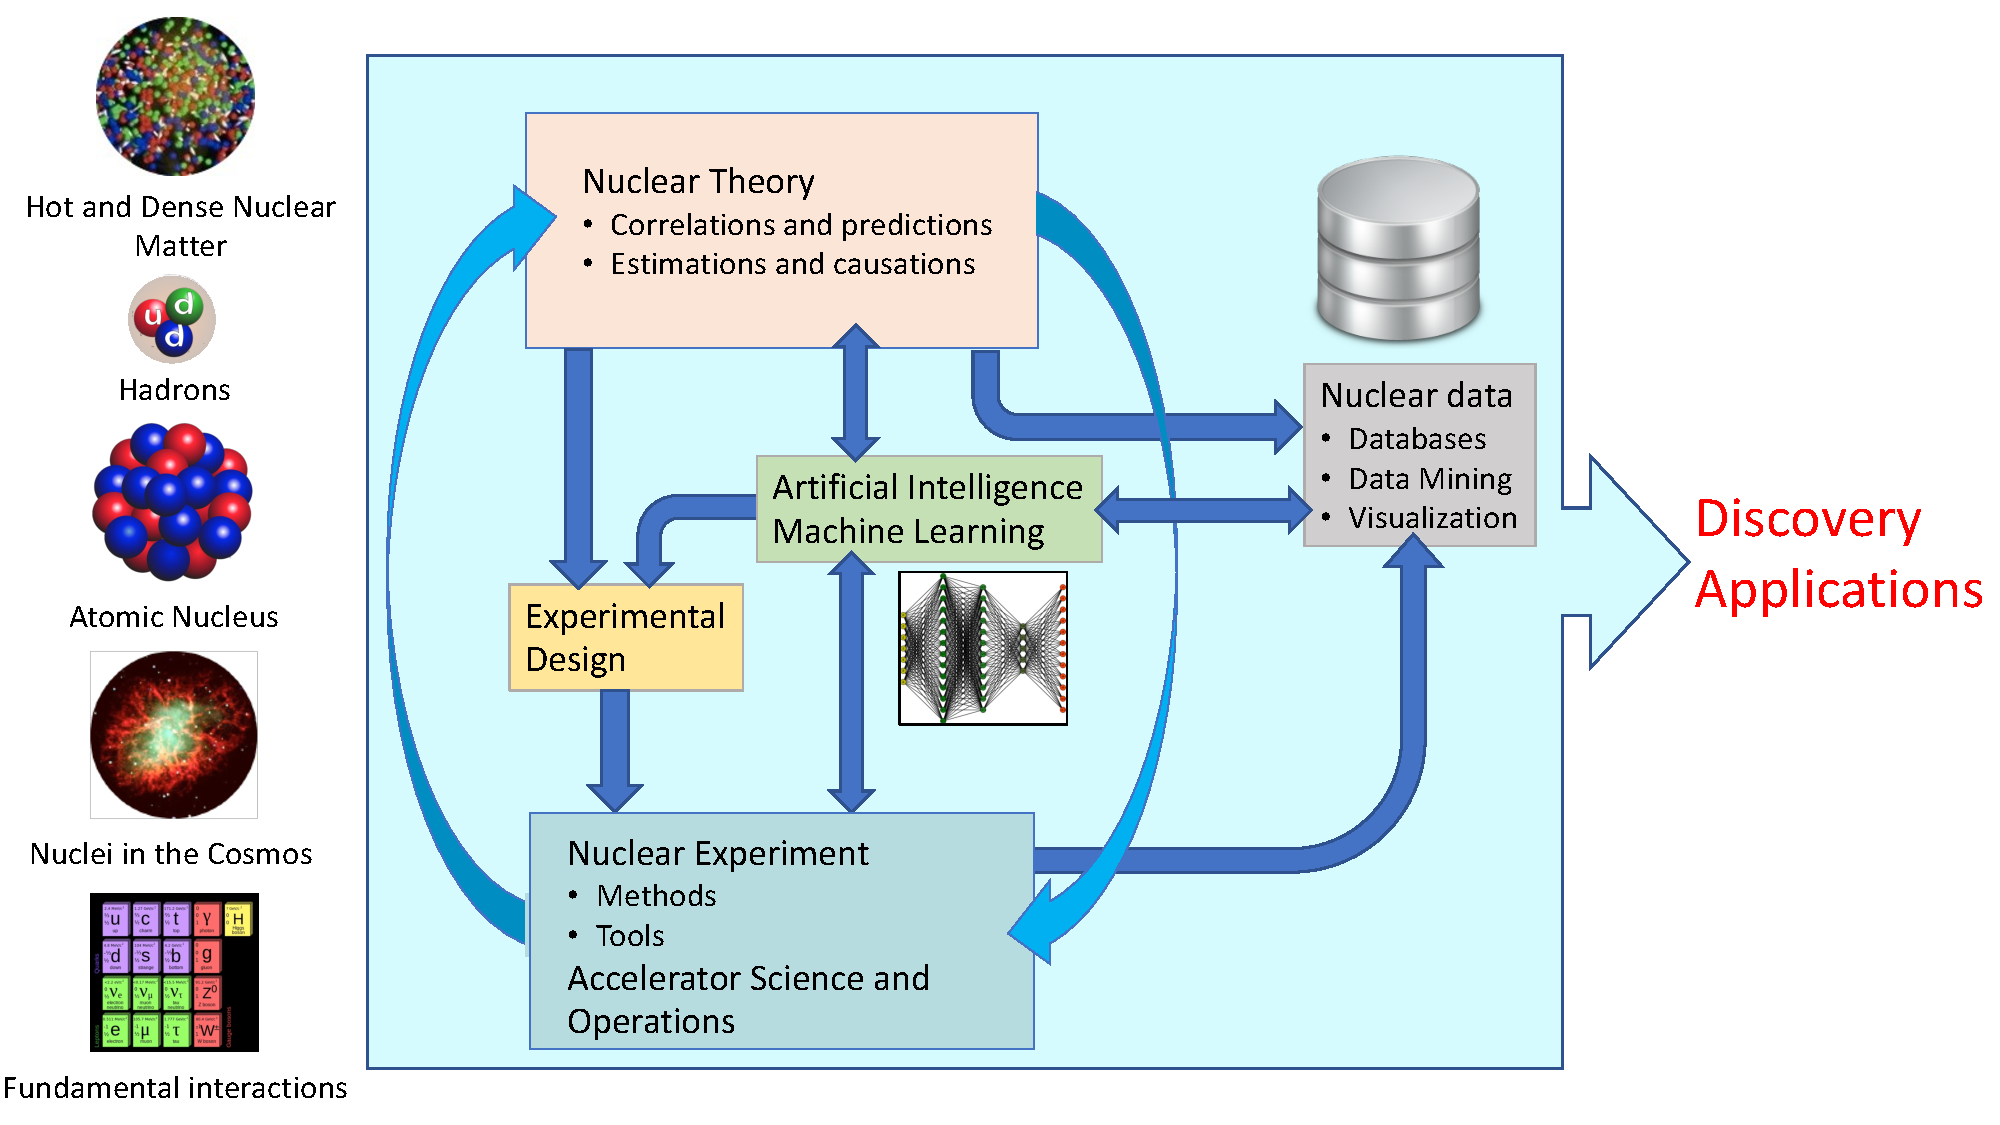
\includegraphics[width=1.0\linewidth]{figures/ML-NP.pdf}}

\vspace{6mm}

% !split
\subsection{AI/ML for the Physical Sciences}

\begin{block}{}
\begin{enumerate}
\item Analyzing data from experiments, see for example from subatomic physics NIMA \href{{https://www.sciencedirect.com/science/article/abs/pii/S0168900221004460?via%3Dihub}}{\nolinkurl{https://www.sciencedirect.com/science/article/abs/pii/S0168900221004460?via\%3Dihub}}

\item Research on quantification of uncertainties

\item Predicting solid state material platforms for quantum technologies, Nature Computational Materials \href{{https://www.nature.com/articles/s41524-022-00888-3}}{\nolinkurl{https://www.nature.com/articles/s41524-022-00888-3}}

\item Solving complicated quantum mechanical many-body systems with deep learning

\item Developing new ML  algorithms \textbf{with applications to quantum computing as well}

\item Research on discriminative and generative AI/ML

\item Computational Neuroscience
\end{enumerate}

\noindent
\end{block}

% !split
\subsection{Scientific Machine Learning}

An important and emerging field is what has been dubbed as scientific ML, see the article by Deiana et al "Applications and Techniques for Fast Machine Learning in Science, Big Data \textbf{5}, 787421 (2022):https://doi.org/10.3389/fdata.2022.787421"

\begin{block}{}
The authors discuss applications and techniques for fast machine
learning (ML) in science -- the concept of integrating power ML
methods into the real-time experimental data processing loop to
accelerate scientific discovery. The report covers three main areas

\begin{enumerate}
\item applications for fast ML across a number of scientific domains;

\item techniques for training and implementing performant and resource-efficient ML algorithms;

\item and computing architectures, platforms, and technologies for deploying these algorithms.
\end{enumerate}

\noindent
\end{block}

% !split
\subsection{ML for detectors}

\vspace{6mm}

% inline figure
\centerline{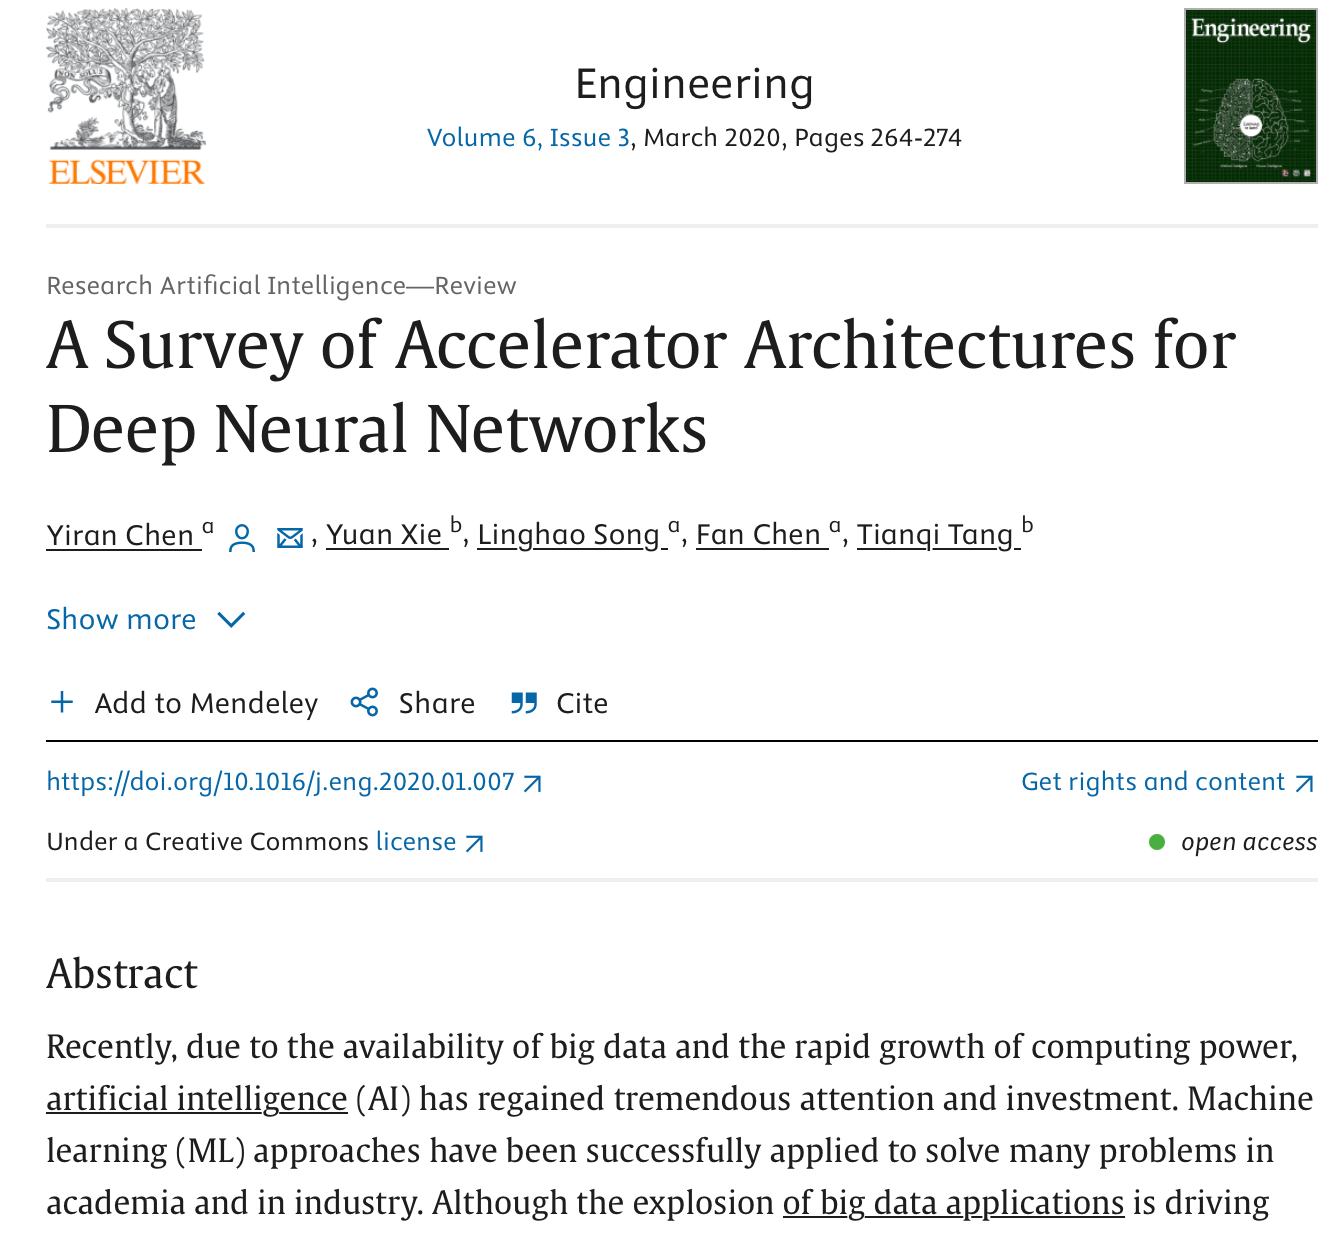
\includegraphics[width=1.0\linewidth]{figures/detectors.png}}

\vspace{6mm}

% !split
\subsection{Physics informed Machine Learning}

Another hot topic is what has loosely been dubbed \textbf{Physics-informed  deep learning}.

It bridges the gap between first-principles based approaches and
data-driven approaches. By incorporating physics information, machine
learning models are encouraged towards solutions that are also
physically meaningful and robust to uncertainties in the data.

See the recent work on "Physics-informed Machine Learning":https://www.nature.com/articles/s42254-021-00314-5".

\begin{block}{Collaborations  }
\begin{enumerate}
\item SINTEF

\item Norwegian Meteorological Institute

\item Simula
\end{enumerate}

\noindent
\end{block}

% !split
\subsection{And more}

\begin{block}{}
\begin{itemize}
\item An important application of AI/ML methods is to improve the estimation of bias or uncertainty due to the introduction of or lack of physical constraints in various theoretical models.

\item In theory, we expect to use AI/ML algorithms and methods to improve our knowledge about  correlations of physical model parameters in data for quantum many-body systems. Deep learning methods show great promise in circumventing the exploding dimensionalities encountered in quantum mechanical many-body studies. 

\item Merging a frequentist approach (the standard path in ML theory) with a Bayesian approach, has the potential to infer better probabilitity distributions and error estimates. 

\item Machine Learning and Quantum Computing is a very interesting avenue to explore. See for example a recent talk by \href{{https://www.youtube.com/watch?v=7WPKv1Q57os&list=PLUPPQ1TVXK7uHwCTccWMBud-zLyvAf8A2&index=5&ab_channel=ECTstar}}{Sofia Vallecorsa}.
\end{itemize}

\noindent
\end{block}

% !split
\subsection{Quantum technologies: what do we have?}

\begin{enumerate}
\item We have at UiO extensive experimental, computational ad theoretical activities in quantum science and technology

\item MiNaLab at UiO is one of the few experimental environments in Norway where we we have a strong research activity on semiconductor based quantum technologies 

\item Quantum sensing is a very active research direction with potential discoveries
\end{enumerate}

\noindent
% !split
\subsection{Five areas of quantum science and technology research in Norway}

\begin{block}{}
\begin{enumerate}
\item Basic quantum science

\item Quantum materials

\item Quantum sensing

\item Quantum communication and cryptography

\item Quantum computing
\end{enumerate}

\noindent
\end{block}

% !split
\subsection{Main academic institutions and centers for basic quantum science}

\begin{block}{UiO }
\begin{enumerate}
\item Physics and CCSE

\item Quantum Chemistry and Hylleraas center
\end{enumerate}

\noindent
\end{block}

\begin{block}{NTNU }
\begin{enumerate}
\item Physics and QSpin center
\end{enumerate}

\noindent
\end{block}

UiB? USN?, UiS?

% !split
\subsection{Quantum materials}

\begin{block}{Universities }
\begin{enumerate}
\item UiO: SMN, LENS, NAFUMA and structure physics

\item NTNU: Physics and QSpin, Department of Electronic Systems
\end{enumerate}

\noindent
\end{block}

\begin{block}{Research institutes and companies (public and private) }
\begin{enumerate}
\item SINTEF

\item Norwegian Metrology Service

\item Norwegian Defense Research Establishment and more
\end{enumerate}

\noindent
\end{block}

% !split
\subsection{Quantum sensing}

\begin{block}{Universities }
\begin{enumerate}
\item UiO: SMN, LENS

\item USN: Quantum technology group
\end{enumerate}

\noindent
\end{block}

\begin{block}{Research institutes and companies (public and private) }
\begin{enumerate}
\item SINTEF

\item Kongsberg group

\item Norwegian Metrology Service

\item Norwegian Defense Research Establishment

\item Equinor, Tomra, Jotne, Sony and more
\end{enumerate}

\noindent
\end{block}

% !split
\subsection{Quantum communication and cryptography}

\begin{block}{Universities }
\begin{enumerate}
\item UiO: Math, Physics and LENS

\item NTNU: Department of Electronic Systems
\end{enumerate}

\noindent
\end{block}

\begin{block}{Research institutes and companies (public and private) }
\begin{enumerate}
\item SINTEF

\item Simula

\item Norwegian Metrology Service

\item Norwegian Defense Research Establishment

\item IBM, Microsoft and other

\item Bank of Norway, DNB, insurance companies and more
\end{enumerate}

\noindent
\end{block}

% !split
\subsection{Quantum computing}

\begin{block}{Universities }
\begin{enumerate}
\item UiO: Math, Physics and CCSE, Quantum Chemistry and Hylleraas

\item NTNU: Qspin

\item OsloMet
\end{enumerate}

\noindent
\end{block}

\begin{block}{Research institutes and companies (public and private) }
\begin{enumerate}
\item SINTEF

\item Simula

\item Norwegian Metrology Service

\item Norwegian Defense Research Establishment

\item IBM, Microsoft and other

\item Bank of Norway, DNB, insurance companies and more
\end{enumerate}

\noindent
\end{block}

% !split
\subsection{Educational strategies}

\begin{enumerate}
\item \textbf{New study direction on Quantum technology} in Bachelor program Physis and Astronomy, starts Fall 2024. Three new courses:
\begin{itemize}

  \item FYS1400 Introduction to Quantum Technologies

  \item FYS3405/4405 Quantum Materials

  \item FYS3415/4415 Quantum Computing

\end{itemize}

\noindent
\item \textbf{Developed Master of Science program on Computational Science}, started fall  2018 and many students here work on quantum computing and machine learning

\item New study direction in Physics Master on Quantum Science and technologies

\item New study direction in Computational Science program on AI and QT

\item Developed courses on machine learning, from basic to advanced ones, FYS-STK3155/4155 and FYS5429/9429

\item Developed advanced course on quantum computing and quantum machine learning, FYS5419/9419

\item Since 2019 organized and taught more than twenty  international schools and intensive courses on quantum computing and machine learning
\end{enumerate}

\noindent
% !split
\subsection{Possible questions for discussions}

\begin{enumerate}
\item How do we incorporate these topics in our education?

\item More difficult: what are the consequences for universities and our educational mission?
\end{enumerate}

\noindent
% !split
\subsection{Education}

\begin{enumerate}
\item Incorporate elements of statistical data analysis and Machine Learning in undergraduate programs

\item Develop courses on Machine Learning and statistical data analysis

\item Build up a series of courses in Quantum Information Technologies (QIT)

\item Modifying contents of present Physics programs or new programs on  Computational Physics and Quantum Technologies
\begin{enumerate}

 \item study direction/option in \textbf{quantum technologies}

 \item study direction/option in \textbf{Artificial Intelligence and Machine Learning}

 \item and more

\end{enumerate}

\noindent
\item Master of Science/PhD programs in Computational and Data Science
\begin{enumerate}

 \item UiO has already MSc programs in CS and DS

 \item Many other universities are developing or have similar programs
\end{enumerate}

\noindent
\end{enumerate}

\noindent
% !split
\subsection{Important Issues to think of}

\begin{enumerate}
\item Lots of conceptual learning: superposition, entanglement, QIT applications, etc.

\item Coding is indispensable. 

\item Teamwork, project management, and communication are important and highly valued

\item Engagement with industry: guest lectures, virtual tours, co-ops, and/or internships.
\end{enumerate}

\noindent
% !split
\subsection{Observations}

\begin{enumerate}
\item Students do not really know what QIT is.

\item ML/AI seen as black boxes/magic!

\item Students perceive that a graduate degree is necessary to work in QIS. A BSc will help.
\end{enumerate}

\noindent
% !split
\subsection{Future Needs/Problems}

\begin{enumerate}
\item There are already  great needs for specialized people (Ph. D. s, postdocs), but also needs of  people with a broad overview of what is possible in ML/AI and/or QIT.

\item There are not enough potential employees in AI/ML and QIT . It is a supply gap, not a skills gap.

\item A BSc with specialization  is a good place to start

\item It is tremendously important to get everyone speaking the same language. Facility with the vernacular of quantum mechanics is a big plus.

\item There is a huge list of areas where technical expertise may be important. But employers are often more concerned with attributes like project management, working well in a team, interest in the field, and adaptability than in specific technical skills.
\end{enumerate}

\noindent

% ------------------- end of main content ---------------

% #ifdef PREAMBLE
\end{document}
% #endif

